% ------------------------------------------------------------------------
% LaTeX Demo:
% ===========
%
%  Graphics Inclusion
%  Color Package Example
%  TeX and International Characters
%  Translation Tables
%  Rotated tables examples
%  Useful TeX-ing Hints
%
% ------------------------------------------------------------------------
% PDFLaTeX this document and view or print it from Acrobat Reader!
% ------------------------------------------------------------------------
% Preamble Starts here:
% ------------------------------------------------------------------------

%\documentclass[reqno]{article}
\documentclass{w-edbk}
\usepackage{ae} % or {zefonts}
\usepackage[T1]{fontenc}
\usepackage[ansinew]{inputenc}
\usepackage{amsmath}
\usepackage{amssymb}
\usepackage{graphicx}
\usepackage{color}
\usepackage[colorlinks]{hyperref}
\usepackage{subfigure}
\usepackage{setspace}


% WinEdt's Bullets ----------------------------------
% Allow WinEdt's Bullets (placeholders) in TeX Files!
% The bullets (eg. in automatically generated tables)
% should be replaced by actual data. In WinEdt you can
% use Ctrl+Space (Tools Menu -> Next Bullet) to navigate
% through bullets and replace them with "real" entries...
\catcode`\=13
\def{$\bowtie$}

% EURO ---------------------------------------
%\usepackage{textcomp} %\texteuro: poor design
%
% Get it from CTAN if it is not included in your TEX distribution
%\usepackage{europs}
%\DeclareInputText{128}{\EUR} % ANSI code for euro: �
%     \EURhv     selects
%     \EURtm     selects EuroSerif
%     \EURcr     selects EuroMono
%     \EUR       selects one of the three above, depending on the current
%                context
%
%     \EURofc    selects EuroSans Regular independent of context
%                N.B.: This is the only "official" Euro symbol. If you
%                      want to conform with the rules of the EU (or
%                      whoever), you may only use this symbol.
%
% HINT: Use MiKTeX's Package Manger to install eurosym package!
\usepackage{eurosym}
\DeclareInputText{128}{\euro} % ANSI code for euro: � \usepackage{eurosym}
\DeclareInputText{165}{\yen}  % ANSI code for yen:  � \usepackage{amssymb}

\usepackage{lscape} %landcape pages support
% Your previewer may not support rotated boxes...
% Rotated boxes are properly displayed in GSView
% and in Adobe's Acrobat Reader

% ------------------------------------------------------------------------
% More TeX Samples and Documentation
% ------------------------------------------------------------------------
%  For more interesting examples check the MiKTeX's "...Doc\MiKTeX"
%  folder. You'll find examples of graphic inclusion, hyper-references,
%  and the use of colors....
%
%  In particular, take a look at:
%
%    epsdemo.tex
%    bmpdemo.tex
%    hyperdemo.tex
%    colordemo.tex
%
%  You'll find out which formats are supported by different conversion
%  utilities, etc...
%
%  Finally, while you are there don't forget to read the MiKTeX.*
%  manual (in your favorite format)!
% ------------------------------------------------------------------------
% Document Starts here:
% ------------------------------------------------------------------------

% FOR DOUBLE SPACING
% \renewcommand{\baselinestretch}{2}

\begin{document}
\title{Person-Specific Characteristic Feature Selection for Face Recognition}
\author [Sreekar Krishna]{SREEKAR KRISHNA\footnote{sreekar.krishna@asu.edu}, VINEETH BALASUBRAMANIAN, JOHN BLACK and SETHURAMAN PANCHANATHAN}
\affil{Center for Cognitive Ubiquitous Computing (CUbiC) \\
School of Computing and Informatics (SCI) \\ Arizona State University \\
Tempe, AZ, USA}

\section{Introduction}
Fingerprint recognition and/or iris recognition have proven to be
very robust when the cooperation of the human subject can be
assumed, both during enrollment and during test.  This makes them
ideal for limiting entry into secured areas (such as buildings) to
known and trusted individuals.  However, these biometrics are not
very useful for recognizing people in public places, where there is
little or no motivation to cooperate with the system.

In contrast, face recognition has the potential for recognizing
people at a distance, without their knowledge or cooperation.  For
decades, banking, retail, commercial, and industrial buildings have
been populated with surveillance cameras that capture video streams
of all people passing through critical areas.  More recently, as a
result of threats to public safety, some public places (such as in
Glasgow and London) have been heavily populated with video
surveillance cameras.  On average, a person moving through London is
captured on video over 5 times a day. This offers an unprecedented
basis for developing and testing face recognition as a biometric for
security and surveillance.

Given this great potential, it is not surprising that many private
corporations have attempted to develop and deploy face recognition
systems, as an adjunct to existing video security and surveillance
systems.  However, the performance of these systems has been
disappointing. Depending on how such a system is adjusted,
miscreants might easily pass through the system undetected, or
innocent people might be incessantly inconvenienced by false alarms.

One of the most difficult problems that face recognition researchers
encounter in surveillance applications is that face databases of
miscreants typically contain only frontal and profile views of each
person's face, with no intermediate views.  Surveillance videos
captured of the same person with the same camera in the same
lighting conditions might have face images that look quite
different, due to pose angle variations, making it very difficult to
compare captured face images to those in a database.  Combine this
problem with the fact that miscreants are highly motivated to
disguise their identity, and the fact that face databases often
contains thousands of faces, and the problem seems insurmountable.

Given all of these complicating factors, it is premature to rely
upon face recognition systems for detecting miscreants in public
places.  On the other hand, the use of face recognition in
controlled access applications (where users are highly motivated to
cooperate, and where face database images can be both captured and
tested with the same camera under the same illumination conditions)
is certainly within the limitations of current face recognition
algorithms.

\subsection{Employing face recognition to facilitate social interactions}
However, there is a real-world application for face recognition that
is moderately challenging, but still potentially within the realm of
possibility. When people who are blind enter a room, they might find
it awkward to initiate social interactions because they don't know
how many people are in the room, who those people are, or where they
are standing \footnote{In order to understand the assistive
technology requirements of people who are blind, we conducted two
focus group studies (one in Tempe, Arizona USA - 9 participants, and
another in Tucson, Arizona USA - 11 participants) which included:
\begin{enumerate} \item students and
adult professionals who are blind,
\item parents of individuals who are blind \item professionals
who work in the area of blindness and visual
impairments\end{enumerate}There was unanimous agreement among
participants that a technology that would help people with visual
impairment to recognize people or hear them described would
significantly enhance their social life.}\hspace*{0.1in}\footnote{To
quote some candidates opinion about face recognition technology in a
social setting:
\begin{itemize}
\item ``It would be nice to walk into a room and immediately get to
know who are all in front of me before they start a conversation''.
\item One young man said, ``It would be great to walk into a bar
and identify beautiful women''.\end{itemize}}. A robust, wearable
face recognition device could solve this problem.

This problem is simplified considerably by the fact that, on a
day-to-day basis most people encounter a limited number of people
whom they need to recognize.  It is further simplified by the fact
that people typically don't attempt to disguise their appearance in
social situations.  When a new person is encountered, the system
could employ face detection to extract and save a sequence of face
images captured during a conversation.  This would provide a wide
variety of facial expressions and pose angles, that could be stored
in a database, and used for training a face recognition algorithm.

As people use such an assistive device over an extended period of
time, they will learn both its abilities and its limitations.
Conjectural information from the system can then be combined with
the user's other sensory abilities (especially hearing) to jointly
ascertain the identity of the person.  This synergy between the user
and the system relaxes some of the stringent requirements normally
placed on face recognition systems.

However, such an assistive technology application still poses some
significant challenges for researchers.  One problem is the extreme
variety of in lighting conditions encountered during normal daily
activities. While there are standards for indoor office lighting
that tend to provide diffuse and adequate lighting, lighting in
other public places might vary considerably. For example, large
windows can significantly alter lighting conditions, and
incandescent lighting is much more yellow than florescent lighting.
Outdoor lighting can be quite harsh in full sunlight, and much more
blue and diffuse in shadows. A person who is blind might not be
aware of extreme lighting conditions, so the system would need to
either (1) be tolerant of extreme variations or (2) recruit the user
to ameliorate those extreme conditions.

In summary, the development of an assistive face recognition system
for people who are blind provides a more tractable problem for face
recognition researchers than security and surveillance applications.
It imposes a somewhat less stringent set of requirements because (1)
the number of people to be recognized is generally smaller, (2)
facial disguise is not a serious concern, (3) multiple pose angles
and facial expressions of a person can be captured as training
images, and (4) the person recognition process can be  a
collaborative process between the system and the user.

In an attempt to provide such an assistive face recognition system,
we have developed a new methodology for face recognition that
detects and extracts unique features on a person's face, and then
uses those features to recognize that person. Contrast this with
conventional face recognition algorithms that might avoid the use of
a few distinguishing features because that approach might make the
system very vulnerable to disguise.

\section{Face Recognition in Humans}
For decades, scientists in various research areas have studied how
humans recognize faces. Developmental psychologists have studied how
human infants start to recognize faces, cognitive psychologists have
studied how adolescents and adults perform face recognition;
neuroscientists have studied the visual pathways and cortical
regions used for recognizing faces, and neuropsychologists have
attempted to integrate knowledge from neurobiological studies with
face recognition research. Computer vision researchers are
relatively new to this area, and have attempted to develop face
recognition algorithms using image processing methods.  Only
recently have computer vision researchers been motivated to better
understand the process by which humans recognize faces, in order to
use that knowledge to develop robust computational models. Their new
interest has lead to more inter-disciplinary face recognition
research, which will likely aid our understanding of face
recognition.

New studies have shown that humans, to a large extent, rely on both
the featural and configural information in face images to recognize
faces ~\cite{Schw2003}. Featural information provides details about
the various facial features, such as the shape and size of the nose,
the eyes, and the chin.  Configural information defines the
locations of the facial features, with respect to each other.
Psychologists Vicki Bruce and Andrew Young ~\cite{Bruce2006} agree
with this dual representation, saying that humans create a
view-centric description of a human face by relying upon
feature-by-feature perceptual input, which is then combined into a
structural model of the face.

Sadar et al ~\cite{Sadr2003} showed that characteristic facial
features are important for recognizing famous faces. For example,
when they erased eye-brows from famous people's faces, face
recognition by human participants was adversely affected.  Young
~\cite{Young1987} showed that human participants were confused when
asked to recognize faces that combined facial features from
different famous faces. These studies suggest that the details of
facial features are important in the recognition of faces.

However, ~\cite{Sinha2006} showed that the relative locations of the
facial features was also very important for the recognition of
faces.  They collected face images of famous personalities, and then
changed the aspect ratio of those images, such that the height was
greatly compressed, while the width was emphasized.  Surprisingly,
all the resulting face images were still recognizable, despite their
contorted appearance, as long as the relative locations of the
features were maintained within the distorted image.  This study
suggests that humans can flexibly use the configural information
when recognizing faces.

Another important area of research in the human perception of faces
has been in understanding the medical condition of face blindness,
called {\it prosopagnosia}.  People with prosopagnosia are unable to
recognize faces including their own. Until recently it was assumed
that prosopagnosia was acquired often as a result of a localized
stroke. However new evidence suggests that a substantial portion of
the general population have a congenital form of prosopagnosia
~\cite{Mccon1976}. Kennerknecht et al ~\cite{Kenner2006} conducted a
survey of 789 students in 2006 which showed that 17 (2.5\%) suffered
from congenital prosopagnosia. These students went about their daily
life without realizing their disorder in face recognition.

Other studies at the Perception research centers at Harvard and Univ
College of London have shown that prosopagnosics recognize people
using unique personal characteristics, such as hair style, gait,
clothing, and voice. These findings suggest that the detection of
unique personal characteristics might provide a basis for face
recognition systems to better recognize people. Since current
methods of face recognition have met with only limited success, it
makes sense to explore the use of this alternative approach.

Research in Own-Race Bias (ORB) in face recognition ~\cite{Turk2005}
has also revealed some interesting results regarding human face
recognition capabilities. David Turk et al. found that, when humans
are presented with new objects or new faces, they initially learn to
recognize those objects and faces based on their distinctive
features.  Then, as familiarity increases, they incorporate
configural information, moving towards holistic recognition. This
study suggests that distinctive features are important during the
initial stages of face recognition, and that configural information
subsequently provides additional useful information.

Distinctive facial features can take many different forms.  For
example, after a first encounter with a person who has a handlebar
moustache, we readily recognize that person by the presence of his
distinctive feature.  Similarly, a person with a large black mole on
her face will be remembered by first-time acquaintances by that
feature.  Given the current limited understanding of how humans
recognize faces, it makes sense to use these observations as the
basis for a new approach to face recognition.

The research described in this chapter is based on the approach of
identifying distinctive facial features that can be used to
distinguish each person's face from other faces in a face database.
In recognition of the role played by configural information in the
later stages of face recognition, it also takes into account the
location of these features with respect to each other.  The results
of our research suggest that this approach can be very effective for
distinguishing one person's face from other faces.

\section{Our Approach to Face Recognition}
Having introduced the potential for using characteristic
person-specific features for face recognition, we now turn our
attention towards the development of a method for discovering such
features, and for using them to index face images. Then we propose a
novel methodology for face recognition, using person-specific
feature extraction and representation. For each person in a face
database, a learning algorithm discovers a set of distinguishing
features (each feature consisting of a unique local image
characteristic, and a corresponding face location) that are unique
to that person. This set of characteristic facial features can then
be compared to the normalized face image of any person, to determine
the presence or absence of those features. Because a unique set of
features is used to identify each person in the database, this
method effectively employs a different feature space for each
person, unlike other face recognition algorithms that assign all of
the face images in the database to a locality in a shared feature
space. Face recognition is then accomplished by a sequence of steps,
in which  query face images is mapped into a locality within the
feature space of each person in the database, and its position is
compared to the cluster of points in that space that represents that
person. The feature space in which the query face images are closest
to the cluster is used to identify the query face images.

Having introduced the conceptual theory behind a person-specific
characteristic feature extraction approach to face recognition, we
now propose in the subsequent sections a method for detecting and
extracting such features from face images, and for constructing a
feature space that is unique to each person in the database.

\section{Feature Extractors}
\subsection{What is a Feature?}
The task of face recognition is inherently a multi-class
classification problem. For every face image $X$, there is an
associated label $y$ that is the name of the class, i.e. the name of
the person depicted in the image. While $X$ represents the image of
the person, there is no inherent constraint on whether the image is
a color RGB, HUV or YCbCr image, or a gray-scale image with a
gray-scale range of 0 to 255, or even spectral representation that
is extracted from the face image using Fourier transform or
Wavelets. Irrespective of the image representation, the basis
vectors spanning that representation are called features. The
feature space spanned by these basis vectors is partitioned  by the
decision boundaries that ultimately define the different classes in
the multi-class problem of face recognition. In this work, we choose
a particular set Gabor filters as feature detectors, and each of
those feature detectors for each person in the database, and that
set of Gabor filters spans a unique feature space for that person.

\subsection{Gabor Features}
\label{subsecGF} Gabor filters are a family of functions (sometimes
called Gabor Wavelets) that are derived from a mother kernel (a
Gabor Function) by varying the parameters of the kernel. As with any
wavelet filters, the Gabor filters extract local spatial frequency
content from the underlying image. Gabor Filters specifically
capture the spatial location and spatial orientation of the
intensity variations in the image underneath the filter's location.
By varying the spatial frequency and the spatial scope of the
filters, it is possible to extract a Gabor coefficient that
partially describes the nature of the image underneath it. The
coefficients obtained by filtering a locality in a face image with a
set of different Gabor Filters are called Gabor Features.

\subsubsection{Use of Gabor Filters in Face Recognition}
Gabor filters have been widely used to represent the receptive field
sensitivity of simple cell feature detectors in the human primary
visual cortex. Recognizing this fact, Gabor features have been
widely used by face recognition researchers. Over the last few
years, the extensive use of Gabor wavelets as generators of feature
spaces for face recognition, has led to objective studies of the
strength of Gabor features for this application. For example, Shan
et al [Shan2004] reviewed the strength of Gabor features for face
recognition using an evaluation method that combined both alignment
precision and recognition accuracy. Their experiments confirmed that
Gabor features are robust to image variations caused by the
imprecision of facial feature localization. As indicated by G�kberk
et al ~\cite{Gokberk2007}, several studies have concentrated on
examining the importance of the Gabor kernel parameters for face
analysis. These include: the weighting of Gabor kernel-based
features using the simplex algorithm for face recognition
~\cite{Wiskott1997}, the extraction of facial subgraphs for head
pose estimation ~\cite{Kruger1997}, the analysis of Gabor kernels
using univariate statistical techniques for discriminative region
finding ~\cite{Kalocsai2000}, the weighting of elastic graph nodes
using quadratic optimization for authentication ~\cite{Tefas2001},
the use of principal component analysis (PCA) to determine the
importance of Gabor features ~\cite{Liu2004}, boosting Gabor
features ~\cite{Yang2004} and Gabor frequency/orientation selection
using genetic algorithms ~\cite{ Wang2002}.

 A relevant work on Gabor Filters for face recognition that is closely related to the
research presented here is by Wiskott and von der Malsburg
~\cite{wiskott_face_1997}. Their work
~\cite{von_der_malsburg_nervous_1985}
~\cite{bienenstock_neural_1987} ~\cite{wiskott_face_1995}
~\cite{wiskott_face_1996},~\cite{wiskott_face_1997} proposes a
framework for face recognition that is based on modeling human face
images as labeled graph. Termed {\em Elastic Bunch Graph Matching}
(EBGM), the technique has become a cornerstone in face recognition
research. Each node of the graph is represented by a group of Gabor
filters/wavelets (called "jets") which are used to model the
 intensity variations around their locations. The edges
of the graph are used to model the relative location of the various
jets. Since the jets represent the underlying image characteristics,
it is desirable to place them on fiducial points on the face. This
is achieved by {\em manually} marking the locations of the facial
fiducial points using a small set of controlled graphs that
represent ``general face knowledge'', which represents an average
geometry for the human face. In our work, a genetic algorithm is
used to obtain the spatial location of the fiducial points. Besides
automating the process of locating these points, our work identifies
spatial locations on the face image that are unique to every single
person, rather than relying on an average geometry.

Closely following the work of Wiskott et. al., Lyons et. al.
~\cite{lyons_automatic_1999} proposed a technique that uses Gabor
Filter coefficients extracted at 1) automatically located
rectangular grid points or 2) manually selected image feature
points. These coefficients are then used to bin face images based on
sex, race and expression. The technique relies on a combined
Principal Component Analysis (PCA) dimensionality reduction and
Linear Discriminant Analysis (LDA) classification over the extracted
Gabor coefficients, to achieve a pooling of images. While the
classification task is not related directly to {\em identifying}
individuals from face images, this technique also demonstrates the
ability of Gabor Filters to extract features that can encode subtle
variations on facial images, providing a basis for face
identification.

\subsubsection{Gabor Filters}
Mathematically, Gabor Filters can be defined as follows:
\begin{equation}
\Psi_{\omega,\theta}  \left(x,y\right) =
\frac{1}{2\pi\sigma_x\sigma_y}\cdot G_\theta\left( x,y\right)\cdot
S_{\omega,\theta}\left(x,y\right) \label{Eqn:GF}
\end{equation}
\begin{equation}
G_\theta\left( x,y\right) = \exp \left\{ - \left( \frac{\left(x \cos
\theta + y \sin \theta \right)^2}{2\sigma_x^2}+\frac{\left(-x \sin
\theta + y \cos \theta \right)^2}{2\sigma_y^2}\right)\right\}
\label{Eqn:G}
\end{equation}
\begin{equation}
S_{\omega,\theta}\left(x,y\right) = \left[\exp \left\{i\left(\omega
x \cos \theta + \omega y \sin \theta \right)\right\} - \exp \left\{-
\frac{\omega^2 \sigma^2}{2} \right\}\right] \label{Eqn:S}
\end{equation}

where,
\begin{itemize}
\item $G_\theta\left( x,y\right)$ represents a Gaussian Function.
\item $S_{\omega,\theta}\left(x,y\right)$ represents a Sinusoid Function.
\item $\left(x,y\right)$ is the spatial location where the filter is centered with respect to the image axis.
\item $\omega$ is the frequency parameter of a 2D Sinusoid.
\item $\sigma^2_{dir}$ represents the variance of the Gaussian (and thus the filter) along the specified direction.
$dir$ can either be $x$ or $y$. The variance controls the region
around the center where the filter has influence.
\end{itemize}

From the definition of Gabor filters, as given in Equation
\ref{Eqn:GF}, it is seen that the filters are generated by
multiplying two components: a Gaussian Function $G_\theta\left(
x,y\right)$ (Equation \ref{Eqn:G}) and a Sinusoid
$S_{\omega,\theta}\left(x,y\right)$ (Equation \ref{Eqn:S}). The
following discussions detail the two components of Equation
\ref{Eqn:GF}.

\subsubsection{Gaussian Function}
The 2D Gaussian function defines the spatial spread of the Gabor
filter. This spread is defined by the variance parameters of the
Gaussian, along the $x$ and $y$ direction together with the
orientation parameter $\theta$. Figure \ref{Fig:G}(a) shows a 3D
representation of the Gaussian mask generated with $\sigma_x = 10$
and $\sigma_y = 15$ and rotation angle $\theta = 0$. The image in
Figure \ref{Fig:G}(b) shows the region of spatial influence of an
elliptical mask on an image, where the variance in the $x$ direction
is larger than the variance in the $y$ direction.

\begin{figure}
\begin{center}
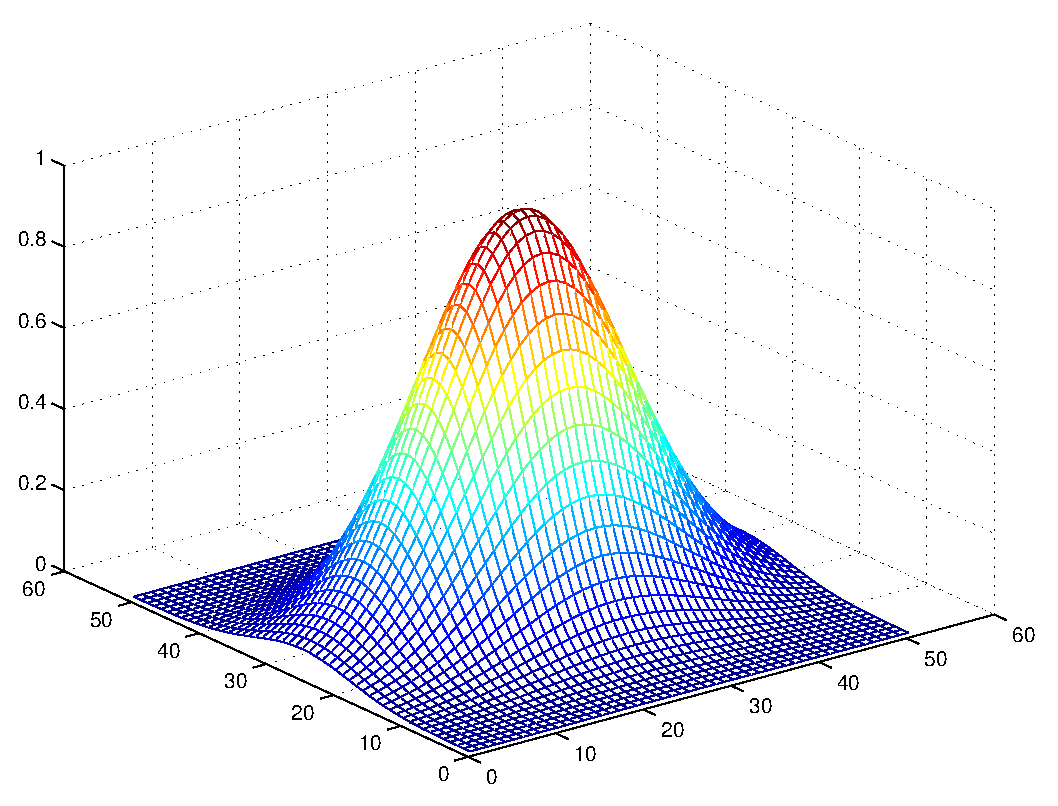
\includegraphics [width=2.3in] {GaussianDiffVar.eps}
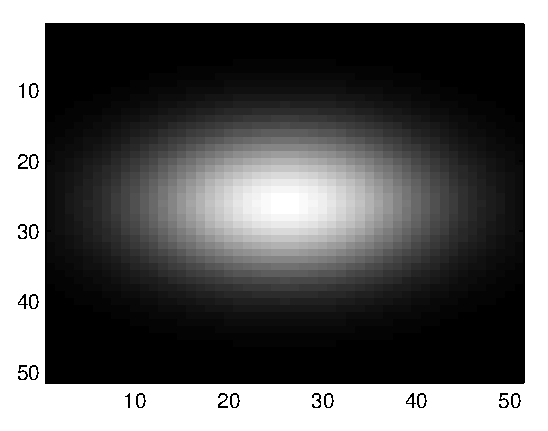
\includegraphics [width=2.3in] {GaussianDiffVarImage.eps}
(a) \hspace{2.25in} (b) \caption{(a) 3D representation of a Gaussian
mask; $\sigma_x = 10$, $\sigma_y = 15$ and $\theta=0$
\newline (b)Image of the Gaussian mask $\sigma_x = 10$, $\sigma_y
= 15$ and $\theta=0$} \label{Fig:G}
\end{center}

\end{figure}


Typically the Gaussian filter has the same variance along both the
$x$ and $y$ directions, that is $\sigma_x = \sigma_y = \sigma$.
Under such conditions the rotation parameter $\theta$ does not play
any role as the spread will be circular.

\subsubsection{Sinusoid}
The 2D complex Sinusoid defined by Equation \ref{Eqn:S} generates
the two Sinusoidal components of the Gabor filters which (when
applied to an image) extracts the local frequency content of the
intensity variations in the signal. The complex Sinusoid has two
components (the real and the imaginary parts) which are two 2D
sinusoids that are phase shifted by $\frac{\pi}{2}$ radians. Figure
\ref{Fig:CS}(a) shows the 3D representation of a Sinusoidal signal
(either real or imaginary) at $\omega = 0.554$ radians and $\theta =
0$ radians, while Figure \ref{Fig:CS}(b) and \ref{Fig:CS}(c) show an
image of the real and imaginary parts of the same complex Sinusoid,
respectively. It can be seen that the two filters are similar,
except for the $\pi$ radian phase shift.

\begin{figure}
\begin{center}
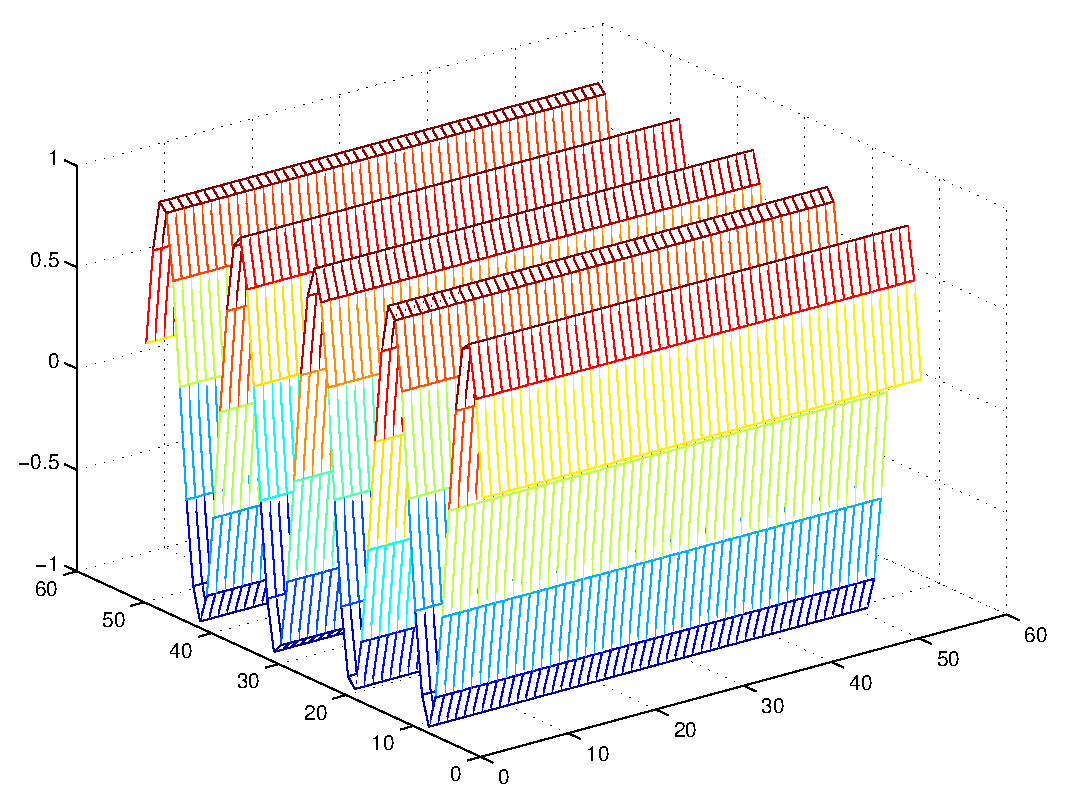
\includegraphics [width=2in] {Sinusoid.eps}
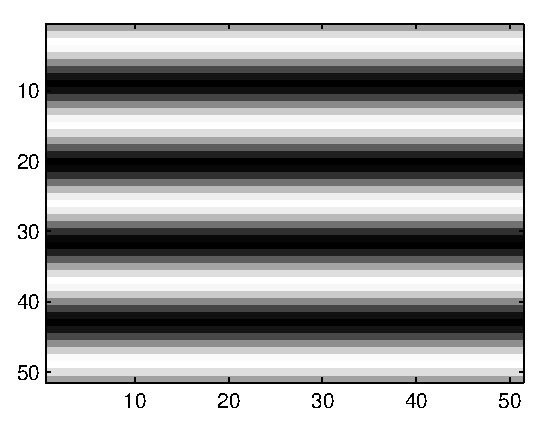
\includegraphics [width=1.25in] {SinusoidRealImage.eps}
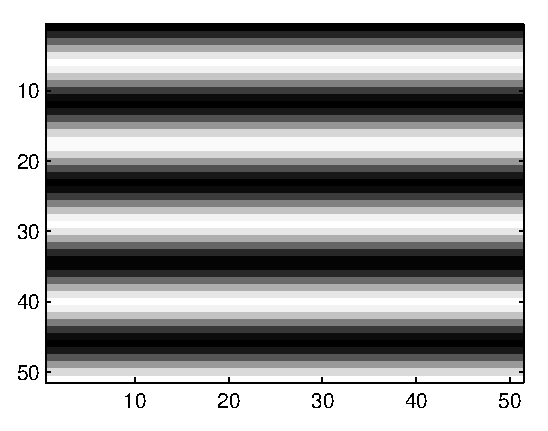
\includegraphics [width=1.25in] {SinusoidImagImage.eps} \newline
(a) \hspace{1.65in} (b) \hspace{1in} (c)

\caption{(a)3D representation of a Sinusoid $S_{\omega,\theta}$
\newline (b)Image representation of the real part of the complex
Sinusoid $\Re\left\{S_{\omega,\theta}\right\}$\newline (c)Image
representation of the imaginary part of complex Sinusoid
$\Im\left\{S_{\omega,\theta}\right\}$} \label{Fig:CS}
\end{center}
\end{figure}

Multiplying the Gaussian and the sinusoid generates the complex
Gabor filter, as defined in Equation \ref{Eqn:GF}. If
$\sigma_x=\sigma_y=\sigma$, then the real and imaginary parts of
this complex filter can be described as follows.

\begin{equation}
\Re\left\{\Psi_{\omega,\theta}  \left(x,y\right) \right\} =
\frac{1}{2\pi\sigma^2}\cdot G_\theta\left( x,y\right)\cdot
\Re\left\{S_{\omega,\theta}\left(x,y\right)\right\}
\end{equation}

\begin{equation}
\Im\left\{\Psi_{\omega,\theta}  \left(x,y\right) \right\} =
\frac{1}{2\pi\sigma^2}\cdot G_\theta\left( x,y\right)\cdot
\Im\left\{S_{\omega,\theta}\left(x,y\right)\right\}
\end{equation}

Figure \ref{Fig:GF}(a) shows the 3D representation of a Gabor filter
(either real or imaginary) at $\omega = 0.554$ radians, $\theta = 0$
radians, and $\sigma = 10$ and Figure \ref{Fig:GF}(b) and
\ref{Fig:GF}(c) show an image with the real and imaginary parts of
the complex filter.

\begin{figure}
\begin{center}
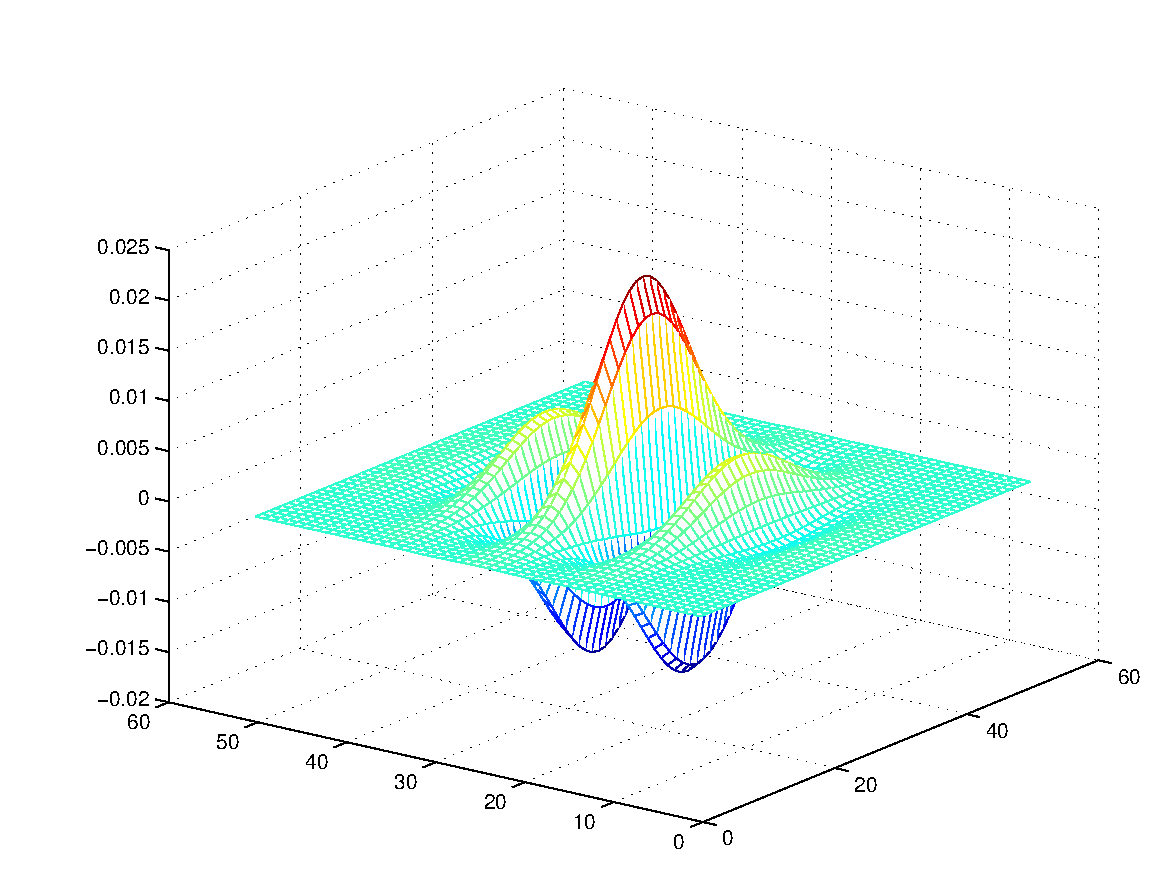
\includegraphics [width = 2in] {GaborFilter.eps}
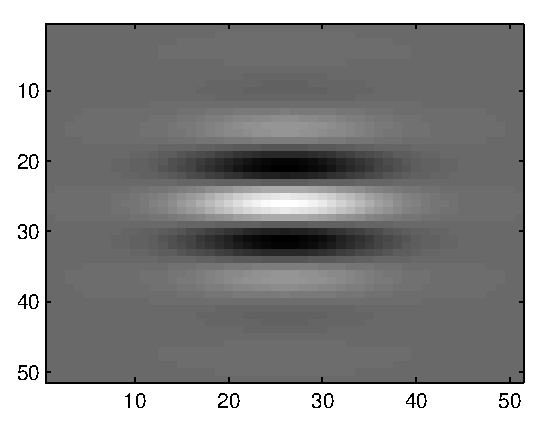
\includegraphics [width = 1.25in] {GaborFilterRealImage.eps}
\includegraphics [width = 1.25in] {GaborFilterImagImage.eps}\newline
(a) \hspace{1.65in} (b) \hspace{1in} (c)


\caption{(a)3D representation of a Gabor filter
$\Psi_{\omega,\theta}$ \newline (b)Image representation of the real
part of Gabor filter  $\Re\left\{\Psi_{\omega,\theta}\right\}$
\newline (c)Image representation of the imaginary part of Gabor filter
$\Im\left\{\Psi_{\omega,\theta}\right\}$} \label{Fig:GF}
\end{center}

\end{figure}

In order to extract a Gabor feature at a location $\left(x,y\right)$
of an image $I$, the real and imaginary parts of the filter are
applied separately to the same location in the image, and a
magnitude is computed from the two results. Thus, the Gabor filter
coefficient at a location $\left(x,y\right)$ in an image $I$ with a
Gabor filter $\Psi_{\omega,\theta}$ is given by
\begin{equation}
C_{\Psi}\left(x,y\right) = \sqrt{\left(I \left(x,y\right) *
\Re\left\{\Psi_{\omega,\theta}\left(x,y\right)\right\}\right)^2 +
\left(I \left(x,y\right) *
\Im\left\{\Psi_{\omega,\theta}\left(x,y\right)\right\}\right)^2}
\label{Eqn:GaborCoeff}
\end{equation}

In our experiments, a {\it Gabor filter bank} was created by varying
three parameters of $\Psi_{\omega,\theta}$: (1) the frequency
parameter $\omega$, (2) the orientation parameter $\theta$, and (3)
the variance parameter $\sigma$. We chose five values for each of
these parameters thereby generating 125 different Gabor filters.

\begin{itemize}
\item $\omega = \left(2^{(-f+2)/2}\cdot \pi\right)$ where, $f =
\{0, 1, 2, 3, 4\}$ \item $\theta = \left(\frac{\pi}{2} \cdot \frac
{1} {5} \cdot t \right)$ where, $t = \{0, 1.25, 2.5, 3.75, 5\}$
\item $\sigma = \{5, 10, 15, 20, 25\}$
\end{itemize}

\section{The Learning Algorithm}
The proposed method uses the above described Gabor filters to find
distinguishing features (and corresponding feature locations) within
a face image. That is, for each person in the database, the
algorithm finds a set of Gabor filters which, when applied at their
corresponding $(x,y)$ locations within the image will produce
coefficients that are unique for that individual. This means that
all of the 125 Gabor filters in the filter bank are applied at each
and every location of each of the individual's face images, and then
tested for their ability to distinguish every individual. Given a
$128 \times 128$ face image, there will be $128 \times 128 \times
125 \times n$ filter coefficients that will be generated per face
image per person, where $n$ is the number of characteristic features
to be extracted for each person. This must be computed for every
person in the training set, which further increases the search
space. To search such a vast space of parameter values (the size of
the Gaussian mask, the frequency of the complex sinusoid, the
orientation of the entire Gabor filter, and the $(x,y)$ location
where the filter is placed) it is important that some scheme for
effective search be incorporated into the system. To this end, we
have chosen Genetic Algorithms to conduct the search. For each
person in the training set, all of the face images that depict to
that person are indexed as positives, while all of the other face
images in the database are indexed as negatives. Dedicated Genetic
Algorithm based search is conducted with these positive and negative
images, with the aim of finding a set of Gabor filters and filter
locations that distinguish all the positives from the negatives.

\subsection{Genetic Algorithms}
When the parameter space is vast (as it is in our case) a Genetic
Algorithm (GA) searches for the optimum solution by randomly picking
parameter sets and evolving newer ones from the best performers.
This happens over many generations, hopefully resulting in the
optimum set of parameters. To start the search, the GA generates a
random set of {\it parents}. Each parent is characterized by the
presence of a {\it chromosome}. The chromosome internally encodes
all the parameters that are used by the parent to perform the
intended operation. In our case, the intended operation is face
recognition. The parent uses the parameters that are found in its
chromosome to derive the Gabor features on the positive and negative
images.

Based on the ability of these features to distinguish a face from
all others in the database, the parent is ranked within its
population. This rank is also referred to as the {\it fitness of the
parent}. The ranking of all the parents, based on their fitness,
marks the end of a generation, and a new generation needs to be
created. New generations are formed based on three important aspects
of GAs, {\it Retention}, {\it Cross Over} and {\it Mutation}. A
portion of the newer generation is derived from the older
generation, using the above mentioned methods, and the rest of the
new generation is created randomly, maintaining the same overall
number of parents between generations. Once a new population has
been formed, the process of ranking parents occurs (as explained
earlier) and a new generation is born out of that ranking. This
iterative process continues until the parents in a certain
generation are fit enough to achieve the given task (with the
desired amount of success) or until the desired number of
generations have evolved.

\subsubsection{Use of Genetic Algorithms in Face Recognition}
GAs have been used in face recognition to search for optimal sets of
features from a pool of potentially useful features that have been
extracted from the face images. Liu et al ~\cite{Liu2002} used a GA
along with Kernel Principal Component Analysis (KPCA) for face
recognition. In their approach, KPCA was first used to extract
facial image features. After feature extraction using the KPCA, GAs
were employed to select the optimal feature subset for recognition -
or more precisely the optimal non-linear components. Xu et al
~\cite{Xu2004} used GAs along with Independent Component Analysis to
recognize faces. After obtaining all the independent components
using the Fast ICA algorithm, a genetic algorithm was introduced to
select optimal independent components.

Wong and Lam ~\cite{Wong1999} proposed an approach for reliable face
detection using genetic algorithms with eigenfaces. After histogram
normalization of face images and computation of eigenfaces, the 'k'
most significant eigenfaces were selected for the computation of the
fitness function. The fitness function was based on the distance
between the projection of a test image and that of the training-set
face images. Since GAs are computationally intensive, the search
space for possible face regions was limited to possible eye regions
alone.

Karungaru et al ~\cite{Karungaru2004} performed face recognition
using template matching. Template matching was performed using a
genetic algorithm to automatically test several positions around the
target, and to adjust the size of the template as the matching
process progressed. The template was a symmetrical T-shaped region
between the eyes, which covered the eyes, nose and mouth.

Ozkan ~\cite{Ozkan2006} used genetic algorithms for feature
selection in face recognition. In this work, the Scale Invariant
Feature Transform (SIFT) ~\cite{lowe_distinctive_2003} was used to
extract features. Since SIFT was originally designed for object
recognition in general, genetic algorithms were used to identify
SIFT features, which are more suitable to face recognition.

Huang and Weschler ~\cite{Huang1999} developed an approach to
identify eye location in face images using navigational routines,
which were automated by learning and evolution using genetic
algorithms. Specifically, eye localization was divided into two
steps: (i) the derivation of the saliency attention map, and (ii)
the possible classification of salient locations as eye regions. The
saliency map was derived using a consensus between navigation
routines that were encoded as finite state automata (FSA) exploring
the facial landscape and evolved using genetic algorithms (GAs). The
classification stage was concerned with the optimal selection of
features and the derivation of decision trees for confirmation of
eye classification using genetic algorithms.

Sun and Yin ~\cite{Sun2005} applied genetic algorithms for feature
selection in 3D face recognition. An individual face model was
created from a generic model and two views of a face. Genetic
algorithms were used to select optimal features from a feature space
composed of geometrical structures, the labeled curvature types of
each vertex in the individualized 3D model.

Sun et al ~\cite{sun2002} approached the problem of gender
classification using a genetic algorithm to select features. A
genetic algorithm was used to select a subset of features from a
low-dimensional representation, which was obtained by applying PCA
and removing eigenvectors that did not seem to encode information
about gender.

As is evident from these citations, many feature-based approaches
towards face recognition use genetic algorithms for feature
selection. However, these approaches employ a single feature space
derived from a set of face images. We believe that it is more
effective to employ aimed at extracting person-specific features,
and that an effective way to do this is by using genetic algorithms.
As observed by \cite{Turk2005}, humans initially learn to recognize
faces based on person-specific characteristic features. This
suggests that better recognition performance might be achieved by
representing each person's face in a person-specific feature space
that is learned using GAs.

The following paragraphs describe how we employed GAs to solve the
problem of finding person-specific Gabor features aimed at face
recognition.

\begin{figure}
\begin{center}
\includegraphics[width = 2in] {chromosome.eps}
\caption{A typical chromosome used in the proposed method.}
\label{Fig:Chromosome}
\end{center}
\end{figure}

\subsubsection{The Chromosome}
Each parent per generation encodes the parameters of a set of Gabor
filters in the form of a chromosome. In our implementation, each
Gabor filter is represented by five parameters. If there are $n$
Gabor filters, parameters for all of these filters are encoded into
the chromosome in a serial manner, as shown in Figure
\ref{Fig:Chromosome}. Thus the length of the chromosome is $5n$. The
number of Gabor filters being used per face image determines the
length of the chromosome. As shown in Figure \ref{Fig:Chromosome},
each parameter in the chromosome is encoded as a gene. The
boundaries of these genes defines the regions where the chromosome
undergoes both the crossover and mutation. The genes can be
considered as the primary element of the parent responsible in the
evolution.

\begin{figure}
\begin{center}
\includegraphics[width = 4in] {firstgeneration.eps}
\caption{Stages in the creation of the first generation of parents}
\label{Fig:FirstGen}
\end{center}
\end{figure}

\subsubsection{Creation of the first generation}
Figure \ref{Fig:FirstGen} depicts the first generation of parents,
which are created randomly. Each parent's chromosome is filled
randomly with parameter values where, each parameter value is within
the allowed range for that parameter. Thus, in our experiment, each
parent potentially has the parameters needed for it to perform face
recognition using Gabor filters for feature extraction.

\begin{figure}
\begin{center}
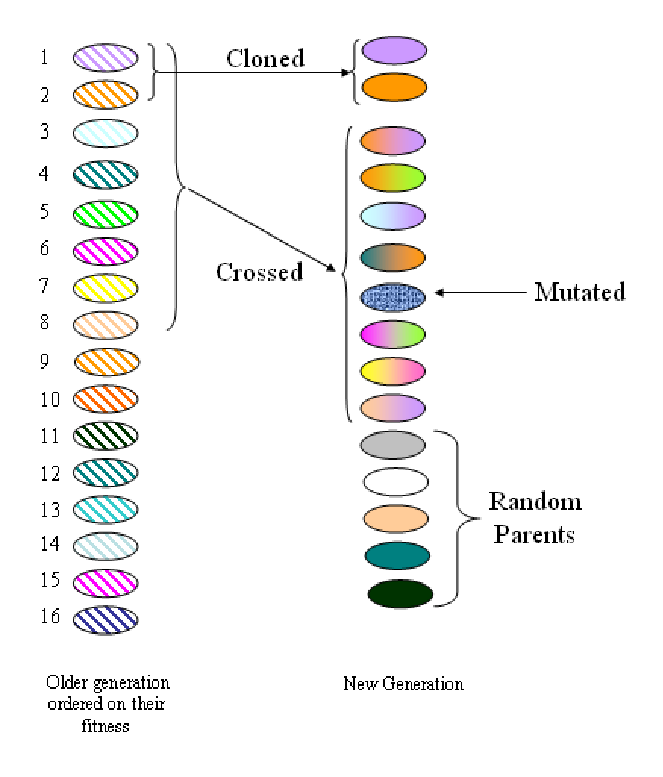
\includegraphics[width = 3in] {latergeneration.eps}
\caption{Deriving newer parents from the current generation}
\label{Fig:laterGen}
\end{center}
\end{figure}

Once these parents are created, each parent in the gene pool is
evaluated based on its capacity to perform face recognition. To this
end, a fitness function is defined, which takes into account the
ability of each parent to distinguish an individual from all others
based on the most distinguishing features on the individual's face.

This fitness function also takes into account the similarity of the
extracted features, and discourages the selection of features that
are highly correlated with each other. This ensures that the face
images will be searched for multiple distinguishing characteristics.
Subsection \ref{Sec:FF} explains in detail the fitness function used
in our experiments. The parents with the best fitness are ranked
higher, and have the highest probability of being picked for using
genetics the next generation. At the end of the rank ordering
process, the parents are arranged in a descending order, based on
their fitness. This rank ordering determines the probability of each
parent being used to create the subsequent generation. If a parent
has a higher fitness, it will have a higher probability of being
cloned into the next generation, or of otherwise being involved in
reproduction.

\subsubsection{Creation of the newer generations}
The newer generations are created from the older population using
{\it clones}, {\it mutants}, and {\it crossovers} of the fittest
parents. To better search for the optimal parameter set, new random
parents are created every generation. This reduces the likelihood
that the algorithm will get stuck in a local minimum in the search
space.

Figure \ref{Fig:laterGen} shows crossover creates a newer
generation, using the fittest parents from the older generation.

The number of offsprings created from mutation, cloning, and
crossover are determined by parameters of the Genetic algorithm. The
number of clones, mutants, and corssovers are controlled by the
following parameters:

\begin{enumerate}
\item {\it Cloning Rate} This parameter controls the number of
parents from the previous generation that will be retained without
undergoing any changes in their genetic structure.
\item{\it Crossover Rate} This parameter controls the number of offsprings that will be
born from crossing the parents from the previous generation.
\item {\it Mutation Rate} This parameter determines how many of the
crossed offsprings will then be mutated.
\item {\it Cloning Distribution Variance} After determining the number of offsprings be to cloned, the
index of the parents for cloning are chosen using a normal
distribution random number generator, with the mean zero and
variance equal to this parameter. Since the parents from the
previous generation have been rank ordered in descending order of
fitness, the zeroth parent will be the top performer (which
coincides with the mean of the random number generator, and has the
highest probability of getting picked).
\item{\it Crossover Distribution Variance} This parameter (which is
similar to the Cloning Distribution Variance) is used to choose the
index of the parents who will undergo Crossover.
\end{enumerate}


\begin{figure}
\begin{center}
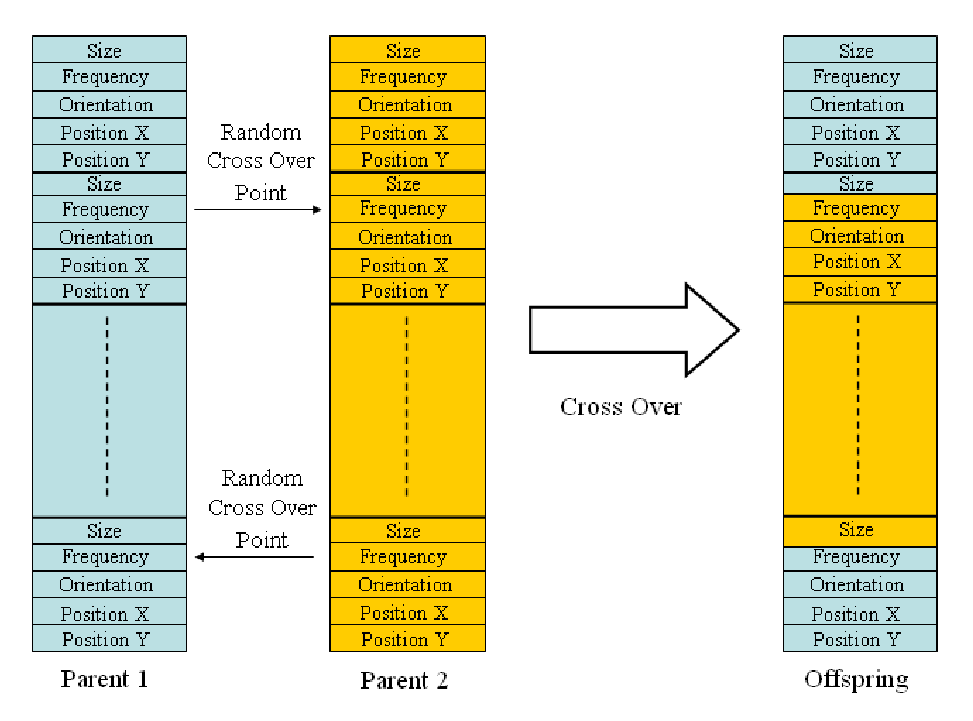
\includegraphics[width = 4in] {crossover.eps}
\caption{Typical crossing of two parents to create an offspring}
\label{Fig:CrossOver}
\end{center}
\end{figure}


\subsubsection{{\it Crossover}}
As discussed earlier, the parents for crossover are selected by a
random number generator. Between these parents, the points of
crossover are determined by choosing locations of crossover
randomly. As seen in the Figure \ref{Fig:CrossOver}, these locations
are arbitrary gene boundary locations and at these locations the
gene content from the two parents gets mixed. The offspring thus
created now contains parts of the genes coming from the contributing
parents. The motivation for this step is the fact that, as more and
more generations pass, the fittest parents undergoing crossover will
already contain the better sets of parameters, and their crossing
might bring together the better sets of parameter values from both
the parents.

\begin{figure}
\begin{center}
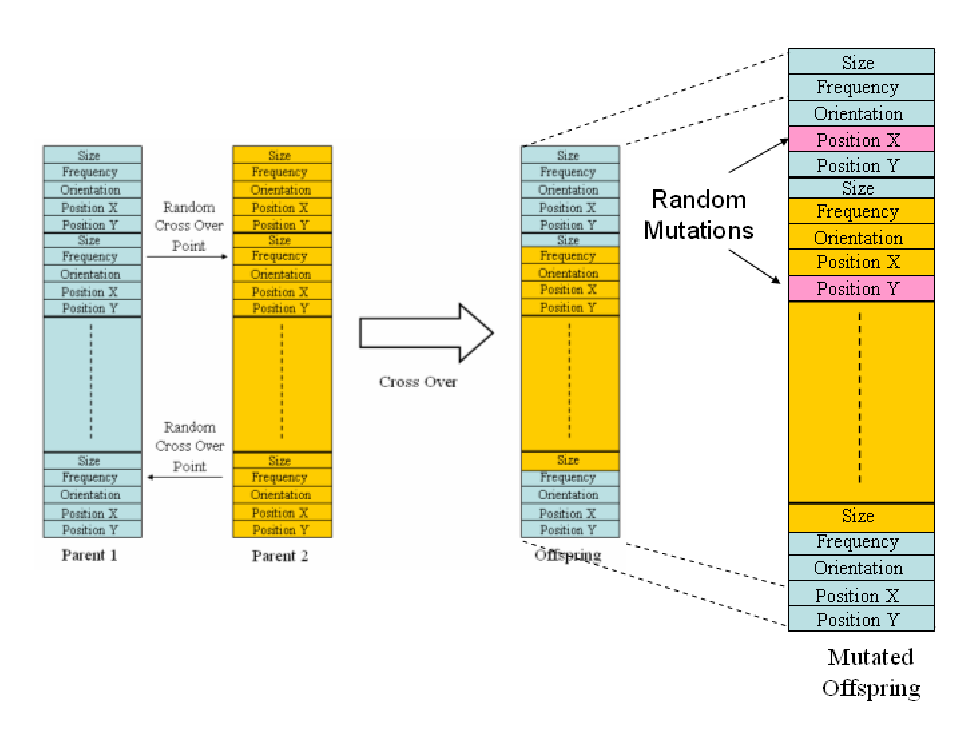
\includegraphics[width = 4in] {mutation.eps}
\caption{Mutation of a newly created offspring} \label{Fig:Mutation}
\end{center}
\end{figure}

\subsubsection{{\it Mutation}}
In addition to the process of crossover at gene boundaries in the
chromosome, the values of some parameters within the genes might be
changed randomly. This is illustrated in the Figure
\ref{Fig:Mutation}. Such mutations help in exploring the local
parameter space more thoroughly. Mutations can be seen as small
perturbations to the larger search that explores the vast parameter
space, searching for the global minima.

\section{Methodology}
Most feature-based face recognition methods use feature detectors
that are not tailored specifically for face recognition, and they
make no attempt to selectively choose feature detectors based
specifically on their usefulness for face recognition. The method
described in this paper uses Gabor wavelets as feature detectors,
but evaluates the usefulness of each particular feature detector
(and a corresponding $(x,y)$ location) for distinguishing between
the faces within our face database. Given the very large number of
possible Gabor feature detectors and locations, we use a Genetic
Algorithm (GA) to explore the space of possibilities, with a fitness
function that propagates parents with a higher ability to
distinguish between the faces in the database. By selecting the
Gabor feature detectors and locations that are most useful for
distinguishing each person from all of the other people in the
database, we define a unique (i.e. person-specific) feature space
for each person.

\subsection{The FacePix (30) Database}
\label{sec:facepix}

All experiments were conducted with face images from the FacePix
(30) database ~\cite{BLACK2002}. FacePix(30) was compiled to contain
face images with pose and illumination angles annotated in 1 degree
increments. Figure \ref{fig-facepix} shows the apparatus that is
used for capturing the face images. A video camera and a spotlight
are mounted on separate annular rings, which rotate independently
around a subject seated in the center. Angle markings on the rings
are captured simultaneously with the face image in a video sequence,
from which the required frames are extracted.

\begin{figure}[h]
    \centering
        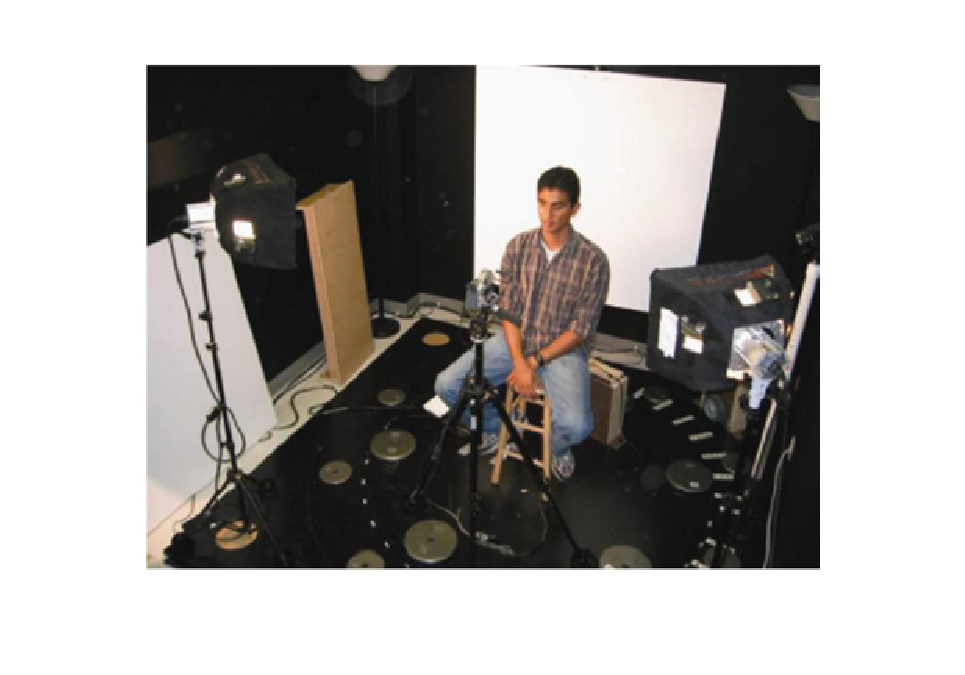
\includegraphics[scale=0.7]{facepix.eps}
    \caption{The data capture setup for FacePix(30)}
    \label{fig-facepix}
\end{figure}

This database has face images of 30 people across a spectrum of pose
and illumination angles. For each person in the database, there are
three sets of images. (1) The {\it pose angle set} contains face
images of each person at pose angles from +90� to �90� (2) The {\it
no-ambient-light set} contains frontal face images with a spotlight
placed at angles ranging from +90� to -90� with no ambient light,
and (3) The {\it ambient-light set} contains frontal face images
with a spot light placed at angles placed at angels from +90� to
-90� in the presence of ambient light. Thus, for each person, there
are three face images available for every angle, over a range of 180
degrees. Figure \ref{fig:facepiximages} provides two examples
extracted from the database, showing pose angles and illumination
angles ranging from -90� to +90� in steps of 10�. For earlier work
using images from this database, please refer ~\cite{Little:2005}.
Work is currently in progress to make this database publicly
available.

\begin{figure}[h]
    \centering
        \includegraphics[width = 4in]{facepiximages.eps}
    \caption{Sample face images with varying pose and illumination from the FacePix(30) database}
    \label{fig:facepiximages}
\end{figure}

We selected at random two images out of each set of three frontal
(0�) (Figure \ref{facepix}) images for training, and used the
remaining image for testing. The genetic algorithms used the
training images to find a set of Gabor feature detectors that were
able to distinguish each person�s face from all of the other people
in the training set. These feature detectors were then used to
recognize the test images.

\begin{figure}[h]
    \centering
        \subfigure[]{
          \label{fig-embeddingsa}
          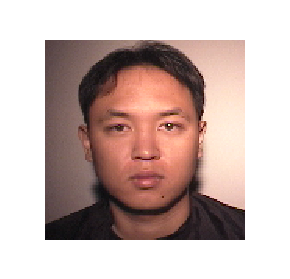
\includegraphics[scale=0.7]{Img1.eps}}
     \hspace{.05in}
     \subfigure[]{
          \label{fig-embeddingsb}
          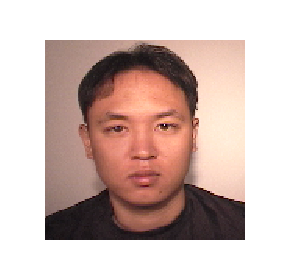
\includegraphics[scale=0.7]{Img2.eps}}
     \hspace{.05in}
     \subfigure[]{
          \label{fig-embeddingsc}
          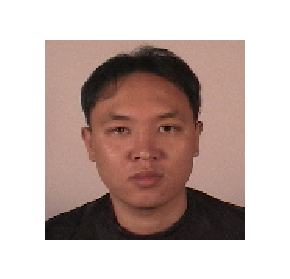
\includegraphics[scale=0.7]{Img3.eps}}
    \caption{Sample frontal images of one person from the FacePix(30) Database}
    \label{facepix}
\end{figure}

In order to evaluate the performance of our system, we used the same
set of training and testing images with face classification
algorithm based on low-dimensional representation of face images
extracted through Principal Component Analysis
~\cite{sirovich_low-dimensional_1987}. Specifically, the performance
of the implementation of PCA-based face recognition followed by
~\cite{Pent1991} was used in our experiments.

\subsection{The Gabor Features}
Each Gabor feature corresponds to a particular Gabor wavelet (i.e. a
particular special frequency, a particular orientation, and a
particular Gaussian-defined spatial extent) applied to a particular
(x, y) location within a normalized face image. (Given that 125
different Gabor filters were generated, by varying $\omega$,
$\sigma$ and $\theta$ in 5 steps each, and given that each face
image contained $128 \times 128 = 16,384$ pixels, there was a pool
of $125 \times 16384 = 2,048,000$ potential Gabor features to choose
from.) We used an N-dimensional vector to represent each person's
face in the database, where N represents the predetermined number of
Gabor features that the Genetic Algorithm selected from this pool.
Figure \ref{fig:facedots} shows an example face image, marked with 5
locations where Gabor features will be extracted (i.e. N = 5). Given
any normalized face image, real number Gabor features are extracted
at these locations using Equation \ref{Eqn:GaborCoeff}. This process
can be envisioned as a projection of a 16,384-dimensional face image
onto an N dimensional subspace, where each dimension is represented
by a single Gabor feature detector.

\begin{figure}
\begin{center}
\includegraphics[scale = 0.5] {Res2.eps}
\caption{A face image marked with 5 locations where unique Gabor
features were extracted} \label{fig:facedots}
\end{center}
\end{figure}

Thus, the objective of the proposed methodology is to extract an N
dimensional real-valued person-specific feature vector to
characterize each person in the database. The N (x, y) locations
(and the spatial frequency and spatial extent parameters of the N
Gabor wavelets used at these locations) are chosen by a GA, with a
fitness function that takes into account the ability of each Gabor
feature detector to distinguish one face from all the other faces in
the database.

\subsection{The Genetic Algorithm}
Every GA is controlled in its progress through generations with a
few control parameters such as,
\begin{itemize}
\item the number of generations of evolution ($n_g$)
\item the number of parents per generation ($n_p$)
\item the number of parents cloned per generation ($n_c$)
\item the number of parents generated through cross over ($n_{co}$)
\item the number of mutations in every generation ($n_m$)
\end{itemize}

In our experiments, the GA used the following empirically-chosen GA
parameters: $n_g = 50$, $n_p = 100$, $n_c=6$, $n_{co}=35$ and
$n_m=5$.

\subsubsection{The Fitness Function \label{Sec:FF}}
The fitness function of a genetic algorithm determines the nature of
the search conducted over the parameter space. For face recognition
applications, the fitness function is the capacity of a parent to
classify the individuals accurately. In our proposed method, the
fitness function needs to take both the Gabor features and the
corresponding feature locations into consideration when evaluating
face classification. We define here a fitness function that has two
components to it. One determines the capacity of the parent to
isolate an individual's face image from the others in the database,
and the other evaluates whether the feature is redundant with other
extracted features (i.e. whether a feature detector produces
coefficients that are highly correlated with the coefficients
produced by another feature detector.) Thus the fitness $F$ can be
defined as

\begin{equation}
F = w_{D} D - w_{C} C \label{Eqn:Fitness}
\end{equation}

where $D$ is the distance measure weighted by $w_{D}$, and $C$
represents the correlation measure which measure the similarity
between the coefficients that have been extracted. The correlation
measure $C$ is weighted by the factor $w_{C}$.

If a parent extracts features from a face image that distinguish one
individual from all the others very well (compared to the other
parents within the same generation) then the distance measure $D$
will be the largest for that parent, making its fitness $F$ large.
If the correlation between the extracted features is small, $C$ will
be small, which also makes the fitness $F$ large. Thus, the
correlation measure serves as a {\it penalty} for extracting the
same feature from the face image multiple times, even though that
particular feature might be the best distinguishing feature on that
face.

The correlation between coefficients was used instead of spatial
separation to counter the problem of similar features being
extracted, because the Gabor filters might not be able to represent
the underlying image characteristic completely. If there are some
large image features on the face (such as beard) that require
multiple Gabor features within a certain spatial locality. Setting a
hard lower limit on this spatial separation might lead to
insufficient representation of that large image feature, in terms of
the Gabor filters.

Consider a parent searching for a unique set of $M$ Gabor filters to
distinguish one individual's face from all other faces. Let this set
of filters be referred to as $S$. Thus, $S = \left\{G_1, G_2,
\cdots, G_M \right\}$ where, $G_m$ represents the $m^{th}$ Gabor
filter.

If the set all individuals in the database is referred to as $I =
\left\{i_1, i_2, \cdots, i_j\right\}$ with $J$ number of
individuals, then for every individual $i$ in $I$ a set $S_i$ has to
be extracted. To achieve this, all the images in the database
depicting individual $i$ are marked as positives, and the ones not
depicting that individual are marked as negatives. Let the set of
positive images be referred to as $P_i$ (with $L$ number of images)
and the set of negatives be referred to as $N$ (with $K$ number of
images). Thus, $S_i = \left\{G_{1i}, G_{2,i}, \cdots, G_{mi}
\right\}$, $P_i = \left\{p_{1i}, p_{2i}, \cdots, p_{li}\right\}$ and
$N_i = \left\{ n_{1i}, n_{2i}, \cdots, n_{ki} \right\}$ are the sets
of Gabor filters, positive images and negatives images set
respectively for the individual $i$.

\begin{itemize}
\item {\bf The Distance Measure} $D$ \\
A parent trying to recognize an individual $i$ with a Gabor filter
set $S_i$ can be thought of as a transformation that projects all of
the face images from the image space to a $M$-dimensional space,
where the dimensions are defined by the $M$ Gabor filters in the set
$S_i$. Thus, all of the images in the two sets $P_i$ and $N_i$ can
be considered as points on this $M$-dimensional space. Since the
goal of the genetic algorithm is to find the set $S_i$ which best
distinguishes the individual $i$ from others, in our method we
search for the $M$ dimensional space (defined by a parent) that best
separates the points formed by the sets $P_i$ and $N_i$. Figure
\ref{Fig:Fitness} is an illustration of hypothetical set of face
images projected on a 2 dimensional space defined by a set of 2
Gabor filters $S_i = \left\{ G_0, G_1 \right\}$. As shown in the
figure, the measure $D$ is the minimum of all the Euclidian
distances between every positive and negative points.

Thus, $D$ can be defined as follow:
\begin{equation}
D = \min_{\forall \hspace{0.09in} l,k} \left[\delta_M
\left(\phi_M(p_{li}), \phi_M(n_{ki})\right)\right]
\end{equation}

where, \\
 $\delta_M (A, B) = \sqrt {(a_1 - b_1)^2 + (a_2 - b_2)^2 +
\cdots + (a_m - b_m)^2}$ is the $M$-dimensional Euclidian distance
between $A$ and $B$. $a_x$ and $b_x$ corresponds the $x^{th}$-coordinate of $A$ and $B$ respectively\\
$\phi_M(X)$ is the transformation function that projects image $X$
from the image space to the $M$-dimensional space defined by the set
of Gabor filters.

\begin{figure}
\begin{center}
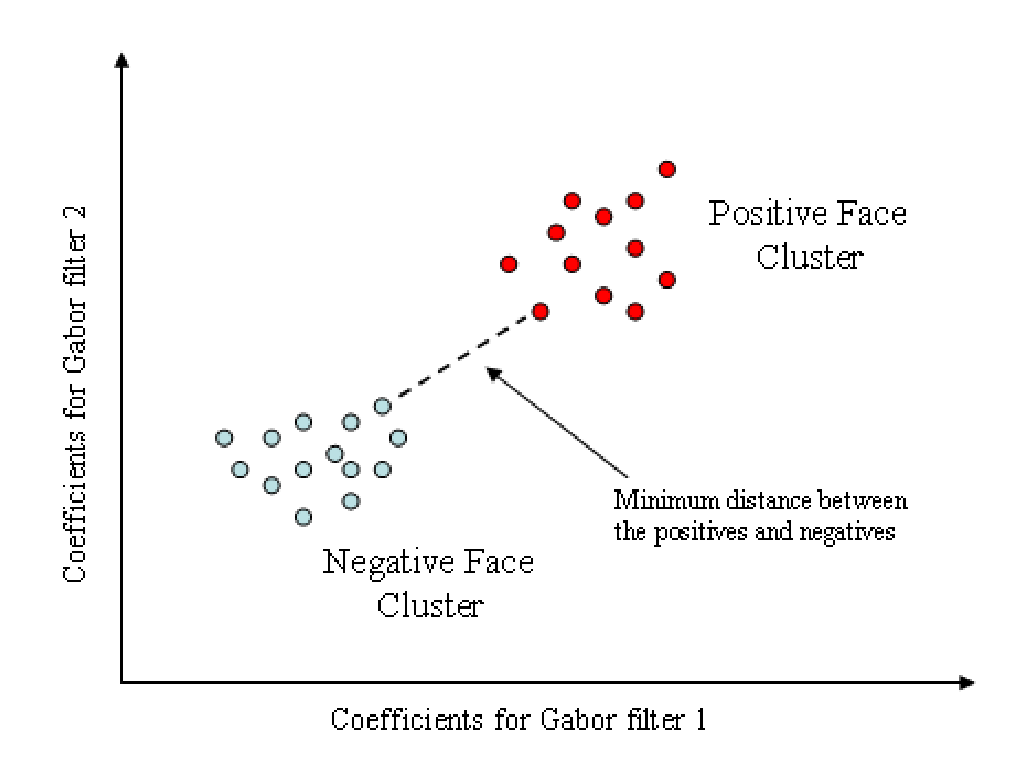
\includegraphics[width = 3in] {fitness.ps}
\caption{Distance Measure $D$ for the fitness function}
\label{Fig:Fitness}
\end{center}
\end{figure}

\item {\bf The Correlation Measure} $C$ \\
In the proposed method, in addition to having every parent selecting
the Gabor filter set $S_i$ that can best distinguish the individual
$i$ from all the others in the database, it is necessary to ensure
that this set of Gabor filters does not include filters that extract
identical image features. If there were no such constraint, the
algorithm might find one very distinguishing image feature on the
face image and, over generations of evolution, all of its Gabor
filters might converge to this one image feature. To avoid this, the
correlation measure $C$ determines the correlation between the image
features extracted at all the locations pointed to by the
chromosome. To test for correlations between the Gabor features at
the different spatial locations, we use the entire set of 125 Gabor
filters to thoroughly characterize the textural context at these
locations.

Assuming that there are $M$ Gabor features that we are looking for
on the face image of individual $i$, let $(x_m, y_m), m = 1, 2,
\dots,M$ be the $M$ points that have been selected genetically in
the chromosome. To find the correlations of the image features
extracted at each of these points, the $N$ Gabor filters $G_i, i =
1, 2, \dots, N$ are used to characterize each of the points. Let the
coefficients of such a characterization be represented by a matrix
$A$. Thus, matrix A is $M \times N$ in dimension, where the rows
correspond to the $M$ locations and $N = 125$ refers to the Gabor
filter coefficients. Thus,

\begin{equation}
A = \left[ \begin{array}{cccc}
g_{(1,1)} & g_{(1,2)} & \ldots & g_{(1,N)}\\
g_{(2,1)} & g_{(2,2)} & \ldots & g_{(2,N)}\\
\vdots  & \vdots  & \vdots & \vdots \\
g_{(m,1)} & g_{(m,2)} & \ldots & g_{(m,N)}
\end{array} \right]
\end{equation}

where, $g_{(m,n)}$ is the coefficient obtained by applying the
$n^{th}$ Gabor filter to the image at the point $(x_m,y_m)$.

The Correlation measure can now be defined in terms of matrix $A$ as
follows

\begin{equation}
C = \log \left(\det \left( diag(B) \right) \right) - \log \left(
\det (B) \right) \label{Eqn:CorrelationMeasure}
\end{equation}

where, $diag (B)$ returns the diagonal matrix corresponding to $B$,
and $B$ is the covariance matrix defined by $B = \frac{1}{N - 1}
(AA^T)$.

Examining the Equation \ref{Eqn:CorrelationMeasure}, it can be seen
that the first log term gets closer to the second log term when the
off diagonal elements of B reduces. The diagonal elements of the
matrix $B$ corresponds to the variance of the $M$ image locations,
whereas the off diagonal elements correspond to the covariance
between pairs if locations. Thus, as the covariance between the
image points decreases, the value of the overall correlation
parameter decreases.

\item {\bf Normalization of} $D$ {\bf and} $C$ \\
In order to have an equal representation of both the Distance
measure $D$ and the Correlation term $C$ in the fitness function, it
is necessary to normalize the range of values that they can take.
For each generation, before the fitness values are used to rank the
parents, parameters $D$ and $C$ are normalized to range between $0$
and $1$.

\begin{eqnarray}
D_{norm} = \frac{D - D_{Min}}{D_{Max} - D_{Min}} \\
C_{norm} = \frac{C - C_{Min}}{C_{Max} - C_{Min}}
\end{eqnarray}

where, the $Max$ represents the maximum value of $D$ or $C$ in a
single generation across all the parents and $Min$ refers to the
minimum value.

\item {\bf Weighting factors} $w_{D}$ {\bf and} $w_{C}$ \\
The influence of the two components of the fitness function are
controlled by the weighting factors $w_{D}$ and $w_{C}$. We used the
relation $w_{C} = 1 - w_{D}$ to control the two parameters
simultaneously. With this relationship, a value of $w_{D} \approx 1$
will subdue the effect of the Correlation measure, causing the
genetic algorithm to choose the Gabor filters on the most prominent
image feature alone. On the other hand, $w_{D} \approx 0$ will
subdue the Distance measure, deviating the genetic algorithm from
the main goal of face recognition. Thus an optimal value for the
weight $w_{D}$ has to be estimated empirically, to suit the face
image database in question.

\end{itemize}

\section{Results}
To evaluate the relative importance of the two terms ($D$ and $C$)
in the fitness function, we ran the proposed algorithm on the
training set several times with 5 feature detectors per chromosome,
while changing the weighting factors in the fitness function for
each run, setting $w_D$  to 0, .25, .50, .75, and 1.00, and
computing $w_C = (1-w_D)$. Figure \ref{RES1} shows the recognition
rate achieved in each case.

\begin{figure}
\begin{center}
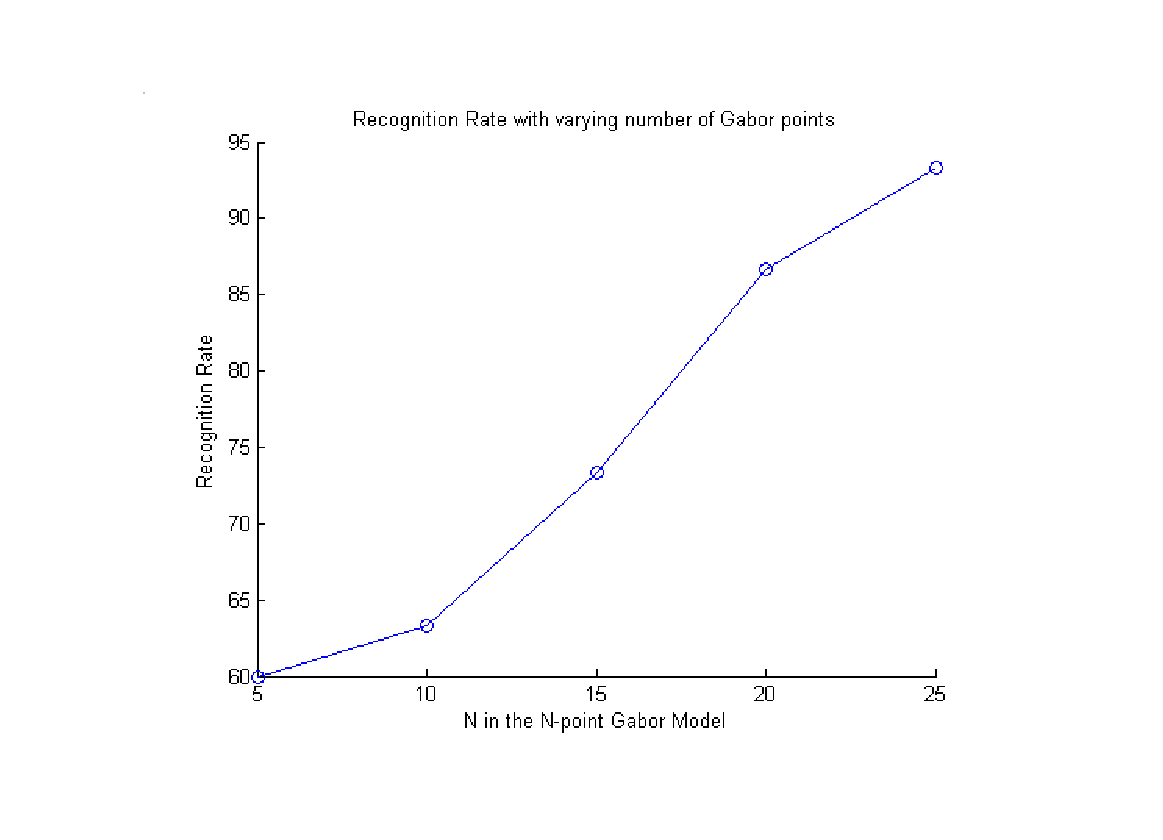
\includegraphics[width = 4in] {Result2.eps}
\caption{The recognition rate versus the number Gabor feature
detectors} \label{RES1}
\end{center}
\end{figure}


We then ran the proposed algorithm on the training set 5 times,
while changing the number of Gabor feature detectors per parent
chromosome for each run to 5, 10, 15, 20, and 25. In all the trials,
$w_D$=0.5. Figure \ref{RES2} shows the recognition rate achieved in
each case.


\begin{figure}
\begin{center}
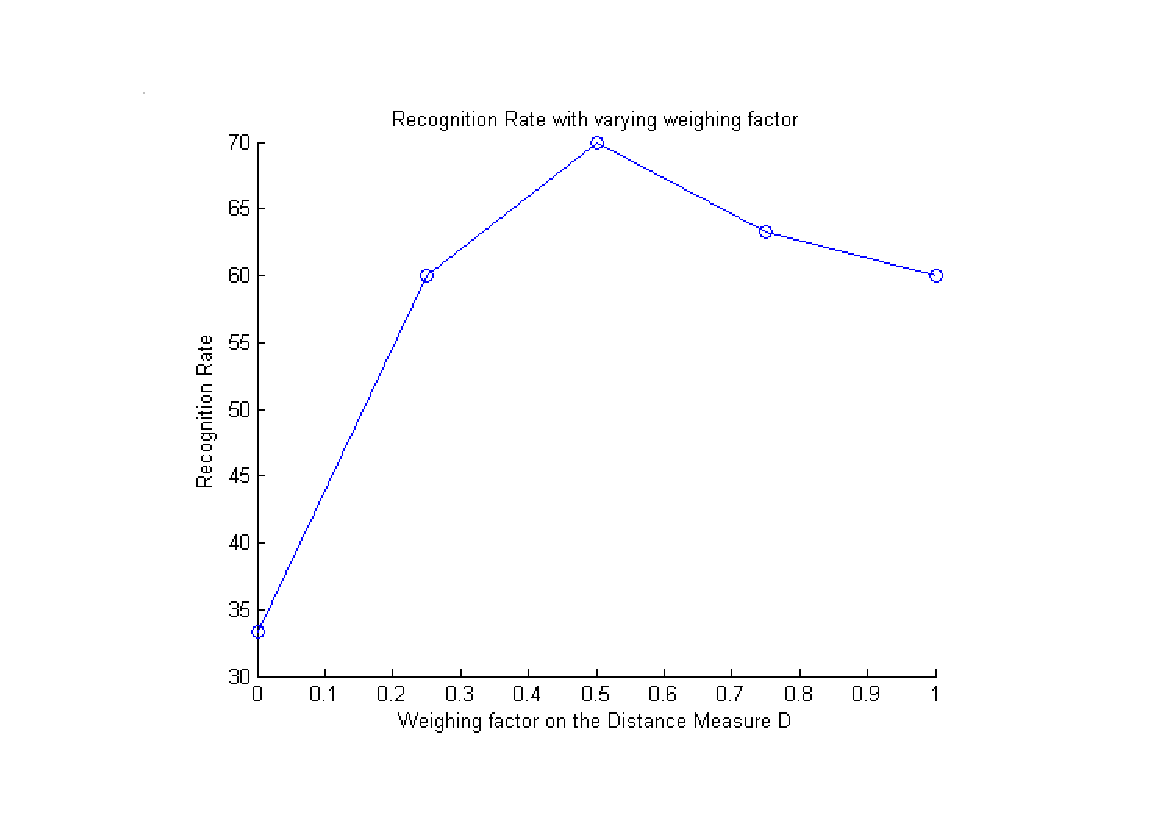
\includegraphics[width = 4in] {Result1.eps}
\caption{Recognition rate with varying $w_D$}\label{RES2}
\end{center}
\end{figure}

\subsection{Discussion of Results}
Figure \ref{RES1} shows that the recognition rate of the proposed
algorithm when trained with 5, 10, 15, 20, and 25 Gabor feature
detectors increases monotonically, as the number of Gabor feature
detectors (N) is increased. This can be attributed to the fact that
increasing the number of Gabor features essentially increases the
number of dimensions for the Gabor feature detector space, allowing
for greater spacing between the positive and the negative clusters.

Figure \ref{RES2} shows that for N = 5 the recognition rate was
optimal when the distance measure D and the correlation measure C
were weighted equally, in computing the fitness function F. The dip
in the recognition rate for $w_D=0.75$ and $w_D=1.0$ indicates the
significance of using the correlation factor C in the fitness
function. The penalty introduced by C ensures that the GA searches
for Gabor features with different textural patterns. If no such
penalty were be imposed, the GA might select Gabor features that are
clustered on one salient facial feature, such as a mole.

The best recognition results for the proposed algorithm (93.3\%)
were obtained with 25 Gabor feature detectors. The best recognition
performance for the PCA algorithm was reached at about 15
components, and flattened out beyond that point, providing a
recognition rate for the same set of faces that was less than
83.3\%. This indicates that, for the face images used in this
experiment (which included substantial illumination variations) the
proposed method performed substantially better than the PCA
algorithm.

\subsection{Person-specific feature extraction}
When the FacePix(30) face database was built, all but one person
were captured without eyeglasses or a hat.  Figures
\ref{fig:result1}(a) and \ref{fig:result1}(b) show the results of
extracting 10 and 20 distinguishing features from that person's face
images. The important things to note about these results are:
\begin{enumerate} \item  At least half of the extracted
Gabor features (8 of the 10) and (10 of the 20) are located on (or
near) the eyeglasses. \item As the number of Gabor features was
increased from 10 to 20, more Gabor features are seen toward the
boundaries of the images. This is due to the fact that the genetic
algorithm chooses Gabor feature locations based on a Gaussian
probability distribution that is centered over the image, and
decreases toward the boundaries of the images.
\end{enumerate}


\begin{figure}[h]
    \centering
        \subfigure[]{
          \label{loga}
          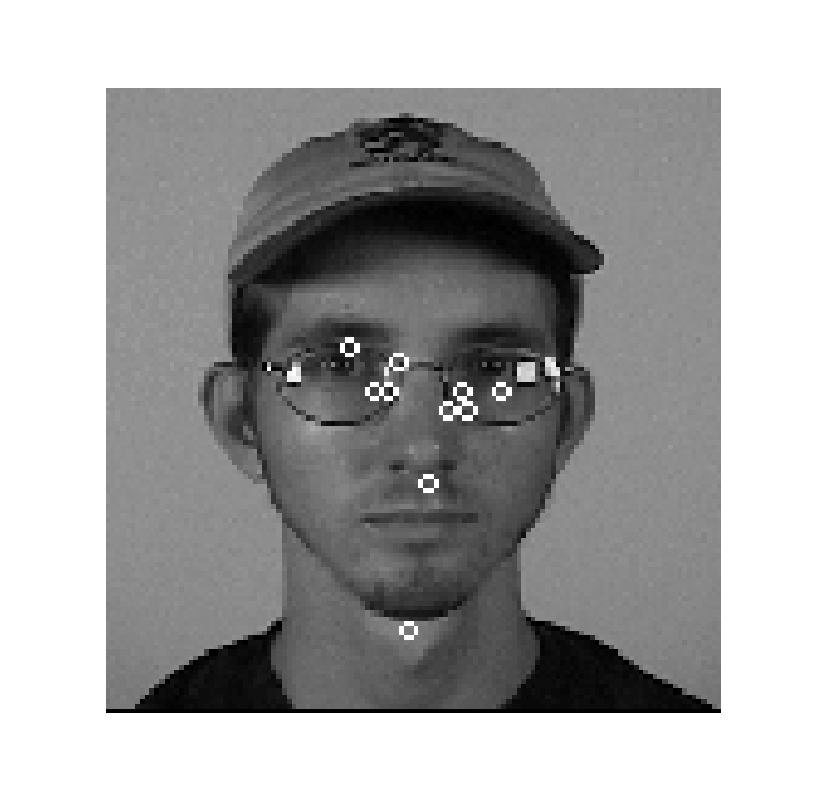
\includegraphics[scale=0.2]{res1.eps}}
          \hspace{.05in}
     \subfigure[]{
          \label{logb}
          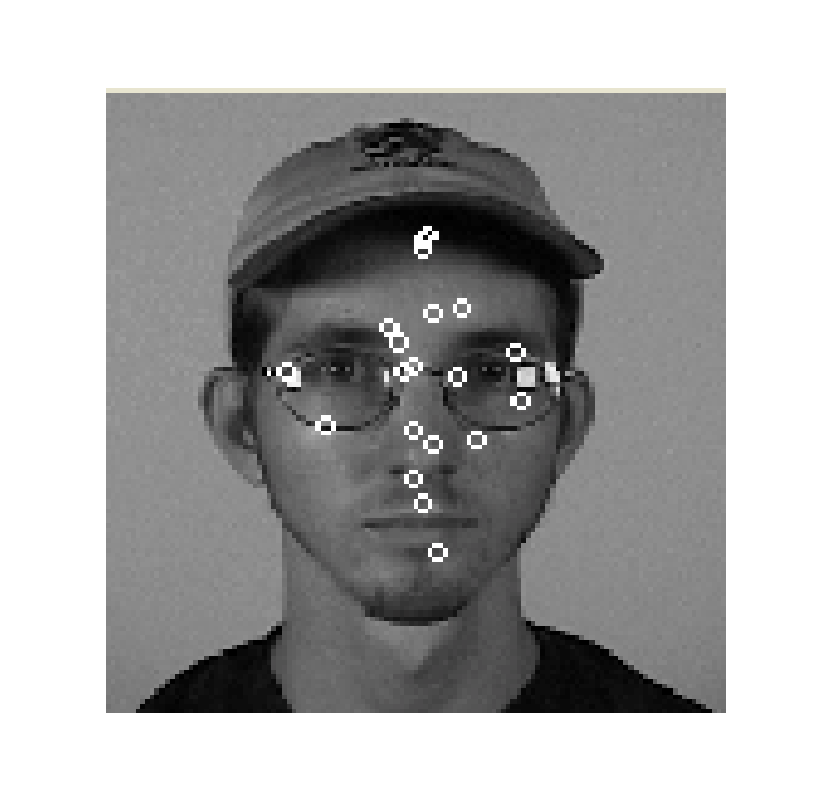
\includegraphics[scale=0.2]{res1b.eps}}
    \caption{10 and 20 person-specific features extracted for a particular individual in the database}
    \label{fig:result1}
\end{figure}

These results suggest that person-specific feature extraction might
be useful for face recognition in small face databases, such as
those typical of a social interaction assistance device for people
who are blind.

\section{Conclusions and Future Work}
As mentioned earlier, the proposed person-specific approach to
evolutionary feature selection in face images is well-suited for
applications such as those that enhance social interaction for
people who are blind, because people do not generally disguise their
appearance in normal social situations, and even when some
significant change occurs (such as a man shaving off his beard) the
system can continue to evolve as it captures new images with each
encounter.

A wearable social interaction assistant prototype has been
implemented using a pair of eyeglasses equipped with a tiny
unobtrusive video camera in the nose bridge ~\cite{Sreekar2005} and
is shown in Figure \ref{Susie}. The analog video output from this
camera is passed through a video digitizer, and the resulting
digital stream is then fed into a portable laptop computer. A video
stream is captured of any person standing in front of the
eyeglasses.  A face detection algorithm, based on Adaboost ~\cite{
violajones01}, is then used to identify the frames of the video
where a face is present, and to localize that face within that
frame. This detected face is then cropped and compared to indexed
faces in a face database.

\begin{figure}[h]
    \centering
        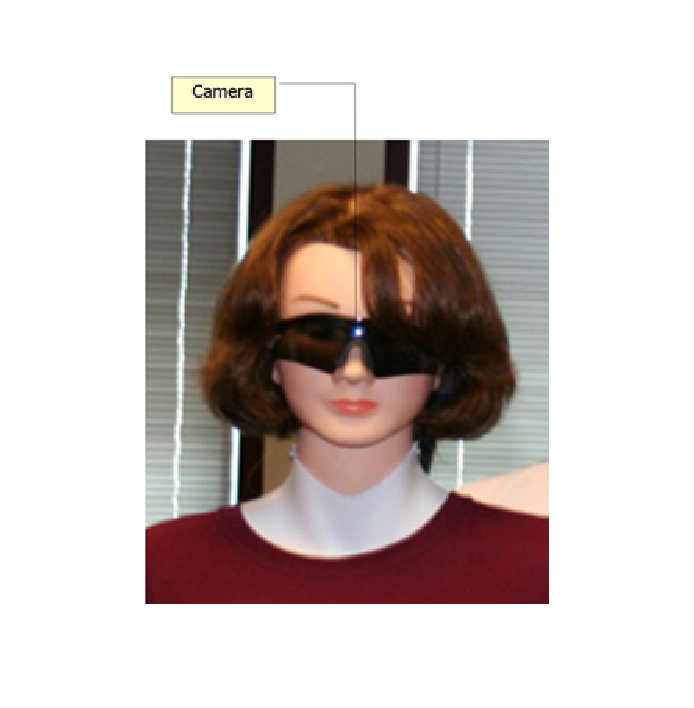
\includegraphics[scale=0.7]{susie.eps}
        \caption{Wearable face recognition platform}
    \label{Susie}
\end{figure}


The performance of the proposed approach for identifying
person-specific features relies, to a large extent, on obtaining
near-frontal views of faces.  To offset this limitation, there is
ongoing work ~\cite{ Balasubramanian2007} to perform
person-independent head pose estimation on the face images obtained
from this platform. It is expected that this will help us select
face images from the video stream with near-frontal views, which
will improve the performance of our algorithm in identifying
person-specific features.

Another factor that limits the performance of our algorithm is
illumination variations in the captured images. Especially
problematic are variations between outdoor-indoor and day-night
settings. (Of course, this limitation is not unique to our
algorithm.) As a strategy to provide additional light unobtrusively
under adverse lighting conditions, we are employing infra-red LED
illuminators in conjunction with an infrared-sensitive camera.

In summary, while there have been many different feature-based
approaches to face recognition over the last two decades of
research, we have proposed a novel methodology based on the
discovery and extraction of person-specific characteristic features
to improve face recognition performance for small face databases.
This approach is aimed at facilitating social interaction in casual
settings. The use of Gabor features, in tandem with a genetic
algorithm to discover characteristic person-specific features has
been inspired by the human visual system and is based on knowledge
that has been developed about the process by which humans recognize
faces.  We believe that more needs to be learnt about human face
recognition, and that as more is learnt, the knowledge can be put to
use to develop more robust face recognition algorithms.

\bibliographystyle{plain}
\bibliography{references}

\end{document}
